\documentclass[11pt]{article}
\usepackage{amsmath,amssymb}
\usepackage{graphicx}

\title{Catalog of Warp-Bubble Shape Functions}
\author{Arcticoder}
\date{May 29, 2025}

\begin{document}
\maketitle

\tableofcontents
\newpage

\section*{Introduction}
This document catalogs candidate warp-bubble shape functions, including their defining formula, support size, and free parameters.
Numeric data for these profiles (r vs f(r)) is available in \texttt{data/profiles.npz} and \texttt{data/profile_data.csv}, generated by the supplied scripts.

\section{Alcubierre Profile}
\subsection*{Defining Formula}
\[
f(r) = \frac{\tanh\bigl(\sigma (r + R)\bigr) - \tanh\bigl(\sigma (r - R)\bigr)}{2\,\tanh(\sigma R)}
\]
\subsection*{Support Size}
Compact support approximately within $r \in [R - \Delta,\, R + \Delta]$, where $\Delta$ depends on $\sigma$.
\subsection*{Free Parameters}
\begin{itemize}
  \item $R$: bubble radius
  \item $\sigma$: steepness parameter
\end{itemize}

\section{Natário Gaussian Variant}
\subsection*{Defining Formula}
\[
f(r) = \exp\!\bigl(-r^2 / \alpha^2\bigr)
\]
\subsection*{Support Size}
Effectively non-compact but decays rapidly; practical support up to $r \approx 3\alpha$.
\subsection*{Free Parameters}
\begin{itemize}
  \item $\alpha$: width parameter
\end{itemize}

\section{Scripts}
The following Python scripts (located in the \texttt{scripts/} folder) support profile visualization and data handling:
\begin{itemize}
  \item \textbf{plot\_profiles.py}: Plot warp-bubble shape functions for visualization.
  \item \textbf{generate\_profile\_data.py}: Generate numeric data for warp-bubble profiles and save to compressed NumPy files.
  \item \textbf{compute\_support\_size.py}: Estimate practical support sizes for profiles given a threshold.
  \item \textbf{export\_profiles\_csv.py}: Export profile data to CSV for further analysis.
\end{itemize}

\section{Visualizations}
Example plot generated by \texttt{plot\_profiles.py}:
\begin{figure}[h]
  \centering
  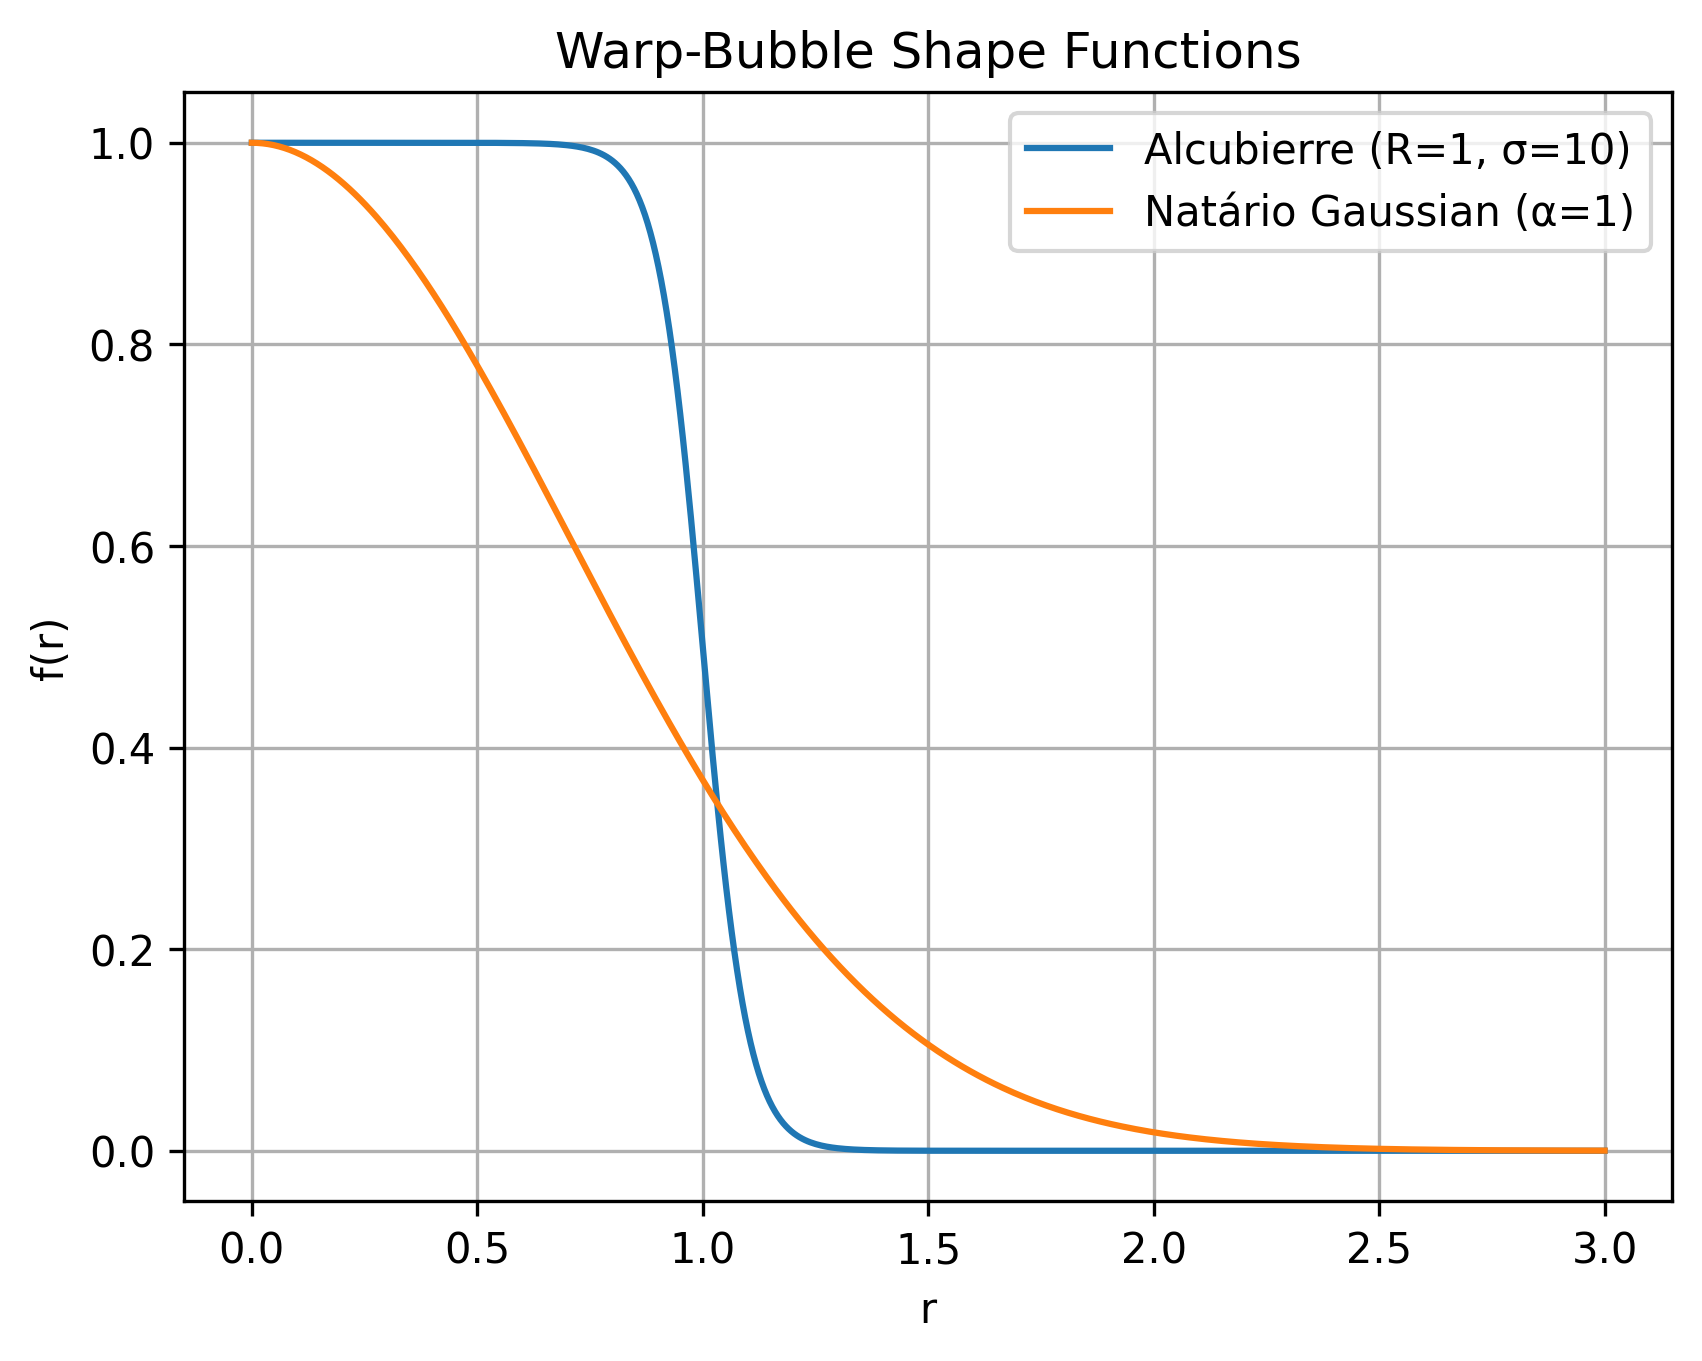
\includegraphics[width=0.7\linewidth]{data/plots/profiles.png}
  \caption{Warp‐bubble profiles generated by \texttt{plot\_profiles.py}.}
\end{figure}

% Add more sections for other profiles here

\end{document}
